%%
%% This is file `sample-manuscript.tex',
%% generated with the docstrip utility.
%%
%% The original source files were:
%%
%% samples.dtx  (with options: `manuscript')
%% 
%% IMPORTANT NOTICE:
%% 
%% For the copyright see the source file.
%% 
%% Any modified versions of this file must be renamed
%% with new filenames distinct from sample-manuscript.tex.
%% 
%% For distribution of the original source see the terms
%% for copying and modification in the file samples.dtx.
%% 
%% This generated file may be distributed as long as the
%% original source files, as listed above, are part of the
%% same distribution. (The sources need not necessarily be
%% in the same archive or directory.)
%%
%% Commands for TeXCount
%TC:macro \cite [option:text,text]
%TC:macro \citep [option:text,text]
%TC:macro \citet [option:text,text]
%TC:envir table 0 1
%TC:envir table* 0 1
%TC:envir tabular [ignore] word
%TC:envir displaymath 0 word
%TC:envir math 0 word
%TC:envir comment 0 0
%%
%%
%% The first command in your LaTeX source must be the \documentclass command.
%%%% Small single column format, used for CIE, CSUR, DTRAP, JACM, JDIQ, JEA, JERIC, JETC, PACMCGIT, TAAS, TACCESS, TACO, TALG, TALLIP (formerly TALIP), TCPS, TDSCI, TEAC, TECS, TELO, THRI, TIIS, TIOT, TISSEC, TIST, TKDD, TMIS, TOCE, TOCHI, TOCL, TOCS, TOCT, TODAES, TODS, TOIS, TOIT, TOMACS, TOMM (formerly TOMCCAP), TOMPECS, TOMS, TOPC, TOPLAS, TOPS, TOS, TOSEM, TOSN, TQC, TRETS, TSAS, TSC, TSLP, TWEB.
% \documentclass[acmsmall]{acmart}

%%%% Large single column format, used for IMWUT, JOCCH, PACMPL, POMACS, TAP, PACMHCI
% \documentclass[acmlarge,screen]{acmart}

%%%% Large double column format, used for TOG
% \documentclass[acmtog, authorversion]{acmart}

%%%% Generic manuscript mode, required for submission
%%%% and peer review
\documentclass[sigconf,screen,review]{acmart}
%% Fonts used in the template cannot be substituted; margin 
%% adjustments are not allowed.
%%
%% \BibTeX command to typeset BibTeX logo in the docs
\AtBeginDocument{%
  \providecommand\BibTeX{{%
    \normalfont B\kern-0.5em{\scshape i\kern-0.25em b}\kern-0.8em\TeX}}}

%% Rights management information.  This information is sent to you
%% when you complete the rights form.  These commands have SAMPLE
%% values in them; it is your responsibility as an author to replace
%% the commands and values with those provided to you when you
%% complete the rights form.
% \setcopyright{acmcopyright}
% \copyrightyear{2026}
% \acmYear{2026}
% \acmDOI{XXXXXXX.XXXXXXX}

%% These commands are for a PROCEEDINGS abstract or paper.
% \acmConference[Conference acronym 'XX]{2026}{Dallas, TX}
%
%  Uncomment \acmBooktitle if th title of the proceedings is different
%  from ``Proceedings of ...''!
%
% \acmBooktitle{Woodstock '18: ACM Symposium on Neural Gaze Detection,
%  June 03--05, 2018, Woodstock, NY} 
% \acmPrice{15.00}
% \acmISBN{978-1-4503-XXXX-X/18/06}


%%
%% Submission ID.
%% Use this when submitting an article to a sponsored event. You'll
%% receive a unique submission ID from the organizers
%% of the event, and this ID should be used as the parameter to this command.
%%\acmSubmissionID{123-A56-BU3}

%%
%% For managing citations, it is recommended to use bibliography
%% files in BibTeX format.
%%
%% You can then either use BibTeX with the ACM-Reference-Format style,
%% or BibLaTeX with the acmnumeric or acmauthoryear sytles, that include
%% support for advanced citation of software artefact from the
%% biblatex-software package, also separately available on CTAN.
%%
%% Look at the sample-*-biblatex.tex files for templates showcasing
%% the biblatex styles.
%%

%%
%% The majority of ACM publications use numbered citations and
%% references.  The command \citestyle{authoryear} switches to the
%% "author year" style.
%%
%% If you are preparing content for an event
%% sponsored by ACM SIGGRAPH, you must use the "author year" style of
%% citations and references.
%% Uncommenting
%% the next command will enable that style.
%%\citestyle{acmauthoryear}

\newcommand{\blue}[1]{{\color{blue}#1}}
\newcommand{\due}[1]{\blue{[FILL FOR {#1}]}}


%%
%% end of the preamble, start of the body of the document source.
\begin{document}

%%
%% The "title" command has an optional parameter,
%% allowing the author to define a "short title" to be used in page headers.
\title{Drift Blindness in AI Models}

%%
%% The "author" command and its associated commands are used to define
%% the authors and their affiliations.
%% Of note is the shared affiliation of the first two authors, and the
%% "authornote" and "authornotemark" commands
%% used to denote shared contribution to the research.

\author{Valentijn Van Overveld}
\authornote{All authors contributed equally to this research.}
\email{vxv200053@utdallas.edu}
\affiliation{%
  \institution{The University of Texas at Dallas}
  \streetaddress{800 W Campbell Rd}
  \city{Richardson}
  \state{TX}
  \country{USA}
  \postcode{75080}
}

\author{Chayanin Noramuttha}
\authornotemark[1]
\email{cxn200002@utdallas.edu}
\affiliation{%
  \institution{The University of Texas at Dallas}
  \streetaddress{800 W Campbell Rd}
  \city{Richardson}
  \state{TX}
  \country{USA}
  \postcode{75080}
}


%%
%% By default, the full list of authors will be used in the page
%% headers. Often, this list is too long, and will overlap
%% other information printed in the page headers. This command allows
%% the author to define a more concise list
%% of authors' names for this purpose.
% \renewcommand{\shortauthors}{Trovato and Tobin, et al.}

%%
%% The abstract is a short summary of the work to be presented in the
%% article.
% \begin{abstract}
% ascascas
% \end{abstract}

%%
%% The code below is generated by the tool at http://dl.acm.org/ccs.cfm.
%% Please copy and paste the code instead of the example below.
%%
% \begin{CCSXML}
% <ccs2012>
%  <concept>
%   <concept_id>00000000.0000000.0000000</concept_id>
%   <concept_desc>Do Not Use This Code, Generate the Correct Terms for Your Paper</concept_desc>
%   <concept_significance>500</concept_significance>
%  </concept>
%  <concept>
%   <concept_id>00000000.00000000.00000000</concept_id>
%   <concept_desc>Do Not Use This Code, Generate the Correct Terms for Your Paper</concept_desc>
%   <concept_significance>300</concept_significance>
%  </concept>
%  <concept>
%   <concept_id>00000000.00000000.00000000</concept_id>
%   <concept_desc>Do Not Use This Code, Generate the Correct Terms for Your Paper</concept_desc>
%   <concept_significance>100</concept_significance>
%  </concept>
%  <concept>
%   <concept_id>00000000.00000000.00000000</concept_id>
%   <concept_desc>Do Not Use This Code, Generate the Correct Terms for Your Paper</concept_desc>
%   <concept_significance>100</concept_significance>
%  </concept>
% </ccs2012>
% \end{CCSXML}

% \ccsdesc[500]{Do Not Use This Code~Generate the Correct Terms for Your Paper}
% \ccsdesc[300]{Do Not Use This Code~Generate the Correct Terms for Your Paper}
% \ccsdesc{Do Not Use This Code~Generate the Correct Terms for Your Paper}
% \ccsdesc[100]{Do Not Use This Code~Generate the Correct Terms for Your Paper}

%%
%% Keywords. The author(s) should pick words that accurately describe
%% the work being presented. Separate the keywords with commas.
% \keywords{Do, Not, Us, This, Code, Put, the, Correct, Terms, for,
%   Your, Paper}

%% A "teaser" image appears between the author and affiliation
%% information and the body of the document, and typically spans the
%% page.
% \begin{teaserfigure}
%   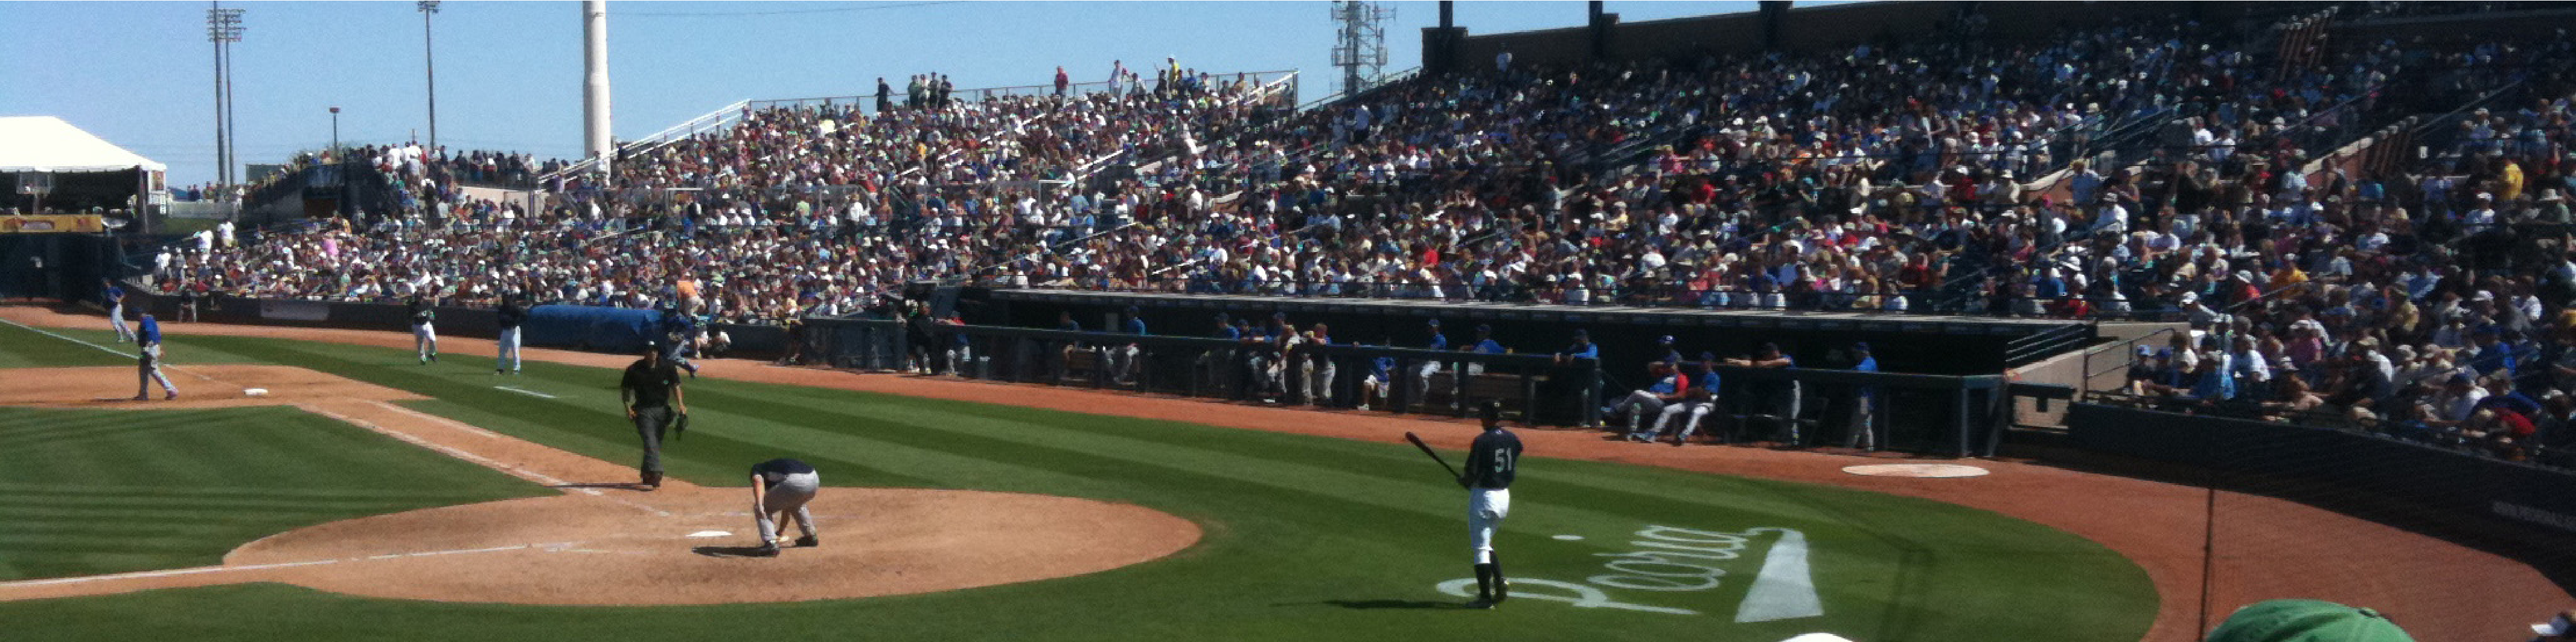
\includegraphics[width=\textwidth]{sampleteaser}
%   \caption{Seattle Mariners at Spring Training, 2010.}
%   \Description{Enjoying the baseball game from the third-base
%   seats. Ichiro Suzuki preparing to bat.}
%   \label{fig:teaser}
% \end{teaserfigure}



%%
%% This command processes the author and affiliation and title
%% information and builds the first part of the formatted document.
\maketitle

\section{Problem}
Throughout the continuous lifecycle of software maintenance and evolution, systems inevitably suffer from architectural drift as the implemented codebase gradually diverges from its prescriptive design constraints. This degradation is introduced by both human developers through ad hoc modifications and by AI coding agents that generate locally correct but structurally harmful code due to their reliance on localized context windows. While recent advances have enabled automated architecture recovery from source code with high accuracy, these approaches remain reactive. They reconstruct architecture after drift has already occurred but provide no mechanism to prevent it from recurring. This project aims to close that gap by automatically translating recovered architectures into enforceable build-time constraints that block violations before they are merged into production.

\section{Motivation}
Addressing architectural drift proactively is critical because unchecked structural degradation quietly accumulates massive technical debt that ultimately paralyzes a system's capacity for long-term maintenance and evolution. This challenge grows more urgent as development teams increasingly adopt autonomous AI coding agents that lack awareness of system-level design constraints. Software architects and maintenance engineers will directly benefit from this research by gaining an automated enforcement pipeline that continuously validates proposed changes against the intended architecture. Consequently, development teams can integrate both human contributors and AI agents into their workflows while preserving the structural integrity and sustainability of their complex systems.

\section{Previous Work}
Recent literature has increasingly explored the intersection of LLMs and software architecture, but efforts to use AI for detecting architectural drift have revealed significant limitations.
\subsection{Exploring Architectural Smells Detection Through LLMs}
Tessa et al.~\cite{tessa2025} investigated the use of off-the-shelf LLMs to detect structural symptoms of drift, such as architectural smells. Specifically, they evaluated Google's Gemini 1.5 Pro on its ability to detect Hub-like Dependencies (HL) in open-source Java projects, comparing its performance against Arcan, a specialized architectural smell detection tool. An HL is a critical smell where a component has excessive incoming and outgoing dependencies.
The study revealed a severe precision and explainability gap. While the LLM achieved 100\% recall in spotting high-dependency components, its precision varied significantly. More detailed prompts improved detection performance from 64\% to 82\% for lower-severity smells, yet the model still could not reliably distinguish architecturally significant dependencies from benign ones. Furthermore, only 49\% of the LLM's explanations for the detected smells were deemed satisfactory by human evaluators. This indicates that the model relies on superficial pattern matching rather than genuine architectural reasoning.

\subsection{Towards Automated Identification of Violation Symptoms of Architecture Erosion}
Li et al.~\cite{li2023} explored the automated identification of architecture erosion by analyzing developer discussions in code reviews. They developed 15 machine learning-based and 4 deep learning-based classifiers using three pre-trained word embeddings to detect violation symptoms from code review comments across four large open-source projects: OpenStack Nova, OpenStack Neutron, Qt Base, and Qt Creator. They further compared these traditional classifiers against LLMs such as GPT-4o, Qwen-2.5, and DeepSeek-R1. The best performing traditional classifier was SVM with word2vec, achieving an F1-score of 0.779.
This approach is fundamentally reactive and dependent on human oversight. It only succeeds when a developer has already noticed the violation and discussed it in a code review comment. Because the classifiers evaluate natural language discussions rather than the underlying structural graph of the codebase, they remain entirely blind to silent drift, which refers to subtle architectural violations that bypass human reviewers during routine feature updates and are never documented in any textual artifact.

\subsection{ArchAgent: Scalable Legacy Software Architecture Recovery with LLMs}
In one of the most advanced attempts to handle large-scale systems, Pan et al.~\cite{pan2026} introduced ArchAgent, a hybrid framework designed to recover architectural design from legacy software. It combines traditional static analysis using Abstract Syntax Trees (ASTs) with LLM-powered semantic synthesis to reconstruct architecture diagrams from cross-repository codebases. In their evaluation across eight large-scale GitHub projects, ArchAgent achieved a mean F1 score of 0.966, demonstrating that accurate architecture recovery from source code is feasible.

However, the authors explicitly highlight the local-scope bias and context limitations of modern LLMs as a primary hurdle. Industrial codebases frequently exceed millions of tokens, which overwhelms the context windows of even the most advanced models. More critically, ArchAgent treats recovery as a one-time diagnostic event. Once the architecture is reconstructed, no mechanism exists to enforce it against future changes, leaving the recovered architecture vulnerable to the same drift that necessitated its reconstruction.

\subsection{Formal Software Architecture Rule Learning: A Comparative Investigation between Large Language Models and Inductive Techniques}
Schindler and Rausch \cite{schindler2024} investigate the use of machine learning techniques to automatically infer software architecture rules from implementation data, addressing the limitations of manual rule specification, which is often time-consuming and error-prone. The study compares inductive rule learning (IRL) approaches with LLMs by applying both to a knowledge base derived from real-world software systems. Their results show that IRL methods, particularly tools like Popper, are generally more effective and consistent in learning rules that align with predefined architectural hypotheses and demonstrate reasonable generalizability across system subsets. In contrast, LLMs exhibit limitations, struggling with formal rule induction, especially when semantic cues are reduced or negative examples are introduced, though they can infer simple rules under favorable conditions. Overall, the paper highlights both the promise and current constraints of data-driven approaches for architectural rule discovery, suggesting that while ML techniques can support more adaptive software architecture practices, further research is needed to improve their robustness and scalability.

Collectively, these studies demonstrate that current approaches face two compounding limitations. First, AI models cannot reliably detect architectural drift natively. They evaluate code locally rather than globally, lack the semantic business context required to distinguish intended design from implemented design, and produce high false-positive rates when evaluating complex structural patterns. Second, even when recovery succeeds with high accuracy, no existing approach translates the recovered architecture into automated, continuous enforcement. Architecture recovery remains a one-time reconstruction rather than an ongoing safeguard, leaving systems vulnerable to recurring drift. This project addresses that gap. While our implementation builds on the ArchAgent repository, it extends prior work, particularly the study by Schindler and Rausch \cite{schindler2024}, by moving beyond rule inference toward integrating learned architectural rules into a continuous enforcement pipeline, bridging the gap between one-time discovery and sustained architectural compliance.


\section{Solution}
We propose an automated enforcement pipeline that translates recovered software architectures into executable build-time constraints, see Figure~\ref{fig:solution}. Our approach takes existing architecture representations and converts them into ArchUnit test rules that continuously validate code changes against the intended design. The pipeline builds on existing architecture documentation to extend the rule-learning approach of Schindler and Rausch \cite{schindler2024}. Rather than stopping at one-time discovery, it converts these architectural rules into continuous, automated enforcement. The main goal is to prevent architectural drift before it is merged into production rather than recovering architecture reactively. 

\begin{figure*}[t]
    \centering
    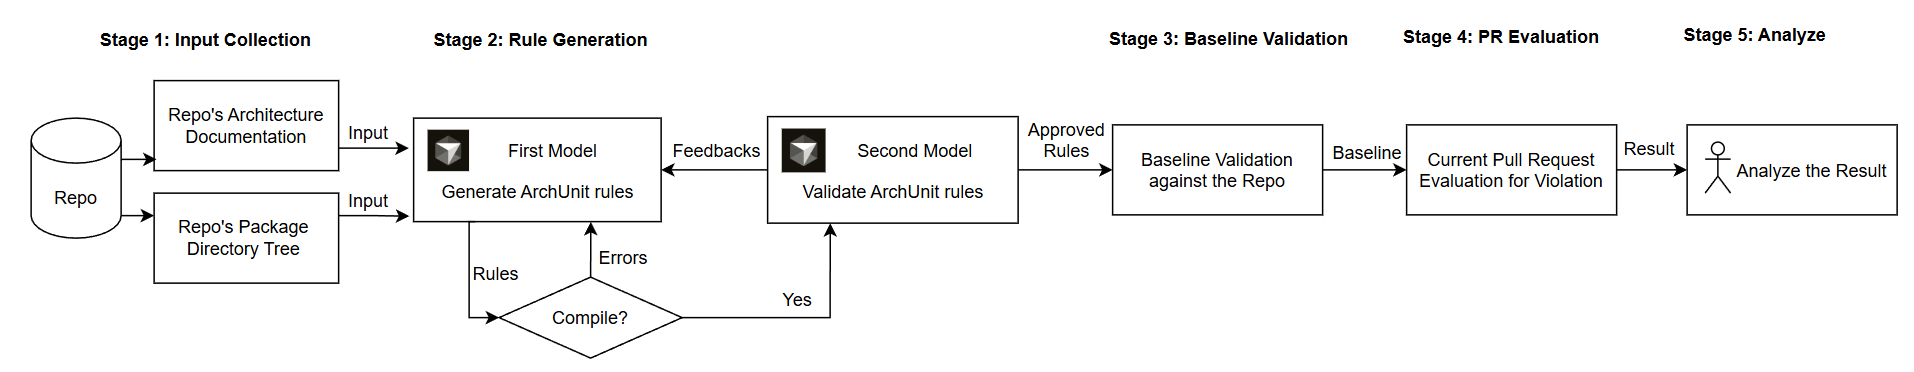
\includegraphics[width=\textwidth]{cs6356 solution.png}
    \caption{Workflow Diagram.}
    \label{fig:solution}
\end{figure*}

\subsubsection{Input}
A set of target software repositories, their package directory structures, and corresponding architecture representations. The architecture representations are sourced from publicly available architectural documentation used as ground truth in the ArchAgent benchmark where available, or from equivalent documentation and recovery outputs for each project. The pipeline is designed to accept any architecture representation, including output from LLM-based recovery tools such as ArchAgent, manually authored documentation, or Mermaid diagrams. The evaluation is conducted across six large-scale, real-world systems: HashiCorp Consul, Spring Framework, Apache ZooKeeper, Kubernetes, Apache Kafka, and Istio. These projects were selected due to their scale, active development, and availability of architectural documentation that can be mapped to their source code structure, enabling a broader assessment of the pipeline’s generalizability beyond a single repository.

\subsubsection{Output}
A set of generated ArchUnit test classes that encode the intended architecture as enforceable dependency constraints, along with a validation report identifying which constraints hold and which are violated across the current codebase and open pull requests.

\subsubsection{Algorithm and Data Transformations}
\begin{enumerate}
    \item Architecture and Structure Collection: The system collects two inputs. First, the architecture representation describing modules, layers, and their allowed dependencies. Second, the repository's package directory tree, extracted via standard file system traversal.
    \item LLM-Based Rule Generation and Cross-Validation: Using the Cursor IDE chat interface, the researcher provides the architecture representation and package directory tree as context and prompts the first model to generate ArchUnit test rules that enforce the documented dependency constraints. The generated rules are then sent to a second, different model along with the original architecture document for adversarial review. The second model verifies that every documented constraint has a corresponding rule, flags any missing or overly broad rules that would trivially pass, and identifies any incorrect package mappings. Feedback from the second model is fed back to the first model for regeneration. The final rules are compiled to verify syntactic correctness, with any compilation failures fed back to the model for self-correction.
    \item Baseline Validation: The generated ArchUnit tests are executed against the current main branch of the repository to establish a clean baseline. Failures are investigated and categorized as either real architectural violations or mapping errors from the generation step.
    \item Pull Request Evaluation: Open pull requests are fetched and checked out locally. The same ArchUnit rules are executed against each PR branch. Any new violations that were not present in the baseline indicate that the PR would introduce architectural drift if merged.
    \item Model Comparison: The rule generation step is repeated using LLMs of varying sizes, such as GPT-4o, Claude Sonnet, and Claude Opus, to evaluate whether smaller, cheaper models can produce equally correct enforcement rules.
\end{enumerate}

\subsubsection{SME Data Incorporated}
The solution incorporates architectural ground truth from public documentation and recovery tools, package-level structural data extracted from the repository, and real pull request data from active open-source development.

\section{Justification}
The technical motivation for this solution stems from a critical gap in the current architecture recovery landscape. As highlighted by Pan et al.~\cite{pan2026}, LLMs suffer from severe local-scope bias and cannot hold an entire system dependency matrix in their context window. Tools like ArchAgent have demonstrated that accurate recovery is achievable despite these limitations, yet recovered architectures carry no enforcement mechanism. Without continuous validation, the same development pressures that caused the original drift will inevitably degrade the recovered architecture again, creating a costly cycle of repeated recovery.

This solution makes sense because it shifts architectural governance from a reactive diagnosis to a proactive safeguard. Previous work by Tessa et al.~\cite{tessa2025} demonstrated that LLMs have poor precision when evaluating architectural patterns and cannot reliably distinguish intended design from problematic structures. Li et al.~\cite{li2023} further showed that detecting violations through developer discussions only captures drift that humans have already noticed. Our approach bypasses both limitations by removing the LLM from the evaluation role entirely. The LLM acts purely as a translator, converting a known architecture into ArchUnit rules. ArchUnit then serves as a deterministic judge, producing strict pass or fail results with no ambiguity and no hallucination risk. This separation of concerns ensures that the accuracy of drift detection depends on the well-established ArchUnit framework rather than on the reasoning capability of any language model.

Additionally, the pipeline incorporates a cross-model validation step in which a second, independent model reviews the generated rules against the original architecture document before execution. This adversarial review ensures that the first model does not produce rules that are overly broad or trivially passing, adding a further layer of separation between generation and evaluation.

Furthermore, by testing the rule generation step across multiple model sizes, this project demonstrates that the enforcement pipeline does not require the expensive large-scale models used in the recovery phase. This makes proactive architectural governance accessible to development teams regardless of their computational resources.

\section{Design and Implementation}
\subsubsection{Type of Tool}
An experimental workflow utilizing the Cursor IDE for LLM-powered rule generation and specific language deterministic architectural validation.

\subsubsection{Technologies}
The Cursor IDE for LLM-based generation of ArchUnit test rules, supporting multiple foundation models such as GPT-4o, Claude Sonnet, and Claude Opus for the model comparison evaluation. ArchUnit for deterministic architectural constraint enforcement. Gradle for compiling and executing the generated test suites against the target Java repositories. Git for fetching and checking out open pull requests during the evaluation phase.

\subsubsection{Architecture}
The workflow consists of four main stages. The Input Collection stage gathers the architecture representation and extracts the package directory tree from the target repository. The Rule Generation stage uses the Cursor IDE chat interface, where the researcher provides the architecture diagram and package structure as context and prompts a first model to generate ArchUnit test classes. A second, different model then reviews the generated rules against the original architecture document to flag missing constraints, overly broad rules, or incorrect package mappings. Feedback is incorporated before final compilation. If the generated code fails to compile, the compilation errors are fed back through Cursor for self-correction. The Baseline Validation stage executes the generated ArchUnit rules against the repository's main branch using Gradle to establish a clean baseline of passing and failing constraints. The PR Evaluation stage fetches open pull requests, checks them out locally, reruns the same ArchUnit rules, and flags any new violations introduced by the proposed changes.

\subsubsection{Interaction Mechanism}
The researcher interacts with the Cursor IDE chat interface to provide architectural context and direct the model to generate ArchUnit rules. The researcher reviews the generated rules for correctness before adding them to the project's test directory. Validation is executed through the terminal using Gradle. For the model comparison evaluation, the researcher repeats the generation step using different foundation models available within Cursor and compares the correctness of the generated rules across model sizes.

\section{Methodology}
\subsection{Evaluation Goal}
To demonstrate that recovered software architectures can be automatically translated into enforceable build-time constraints that detect architectural drift in both human-written and AI-generated code changes before they are merged into production.

\subsection{Research Questions}
\begin{enumerate}
    \item RQ1: Can LLMs accurately translate a recovered architecture representation into correct and compilable ArchUnit rules that reflect the intended dependency constraints?
    \item RQ2: Do the generated ArchUnit rules successfully detect architectural violations in open pull requests against the target repositories?
    \item RQ3: Does the accuracy of the generated rules vary significantly across LLMs of different sizes, and can smaller, cheaper models produce enforcement rules of comparable quality to larger models?
\end{enumerate}

\subsection{Success Criteria}
    \begin{enumerate}
    \item RQ1 will be considered positively answered if the generated ArchUnit rules achieve a Compilation Success Rate above 90\% after the self-correction loop and a Rule Generation Accuracy above 80\% when compared against a manually verified reference set of architectural constraints.
    \item RQ2 will be considered positively answered if the generated rules successfully identify at least one legitimate architectural violation in an open pull request that was not present in the main branch baseline. If no violations are found in existing pull requests, the pipeline must detect a deliberately introduced cross-layer dependency in a controlled fork, confirming that the enforcement mechanism functions as intended.
    \item RQ3 will be considered positively answered if the smallest model tested achieves a Rule Generation Accuracy within 10 percentage points of the largest model, demonstrating that the enforcement step does not require expensive large-scale models.
\end{enumerate}

\subsection{Datasets}
Six repositories selected from the benchmark projects evaluated in the ArchAgent study. These repositories have verified architectural ground truth, span multiple domains such as distributed systems, web frameworks, and data processing, and range from approximately 1,000 to 22,000 source files.

\subsection{Metrics}
\begin{itemize}
    \item Rule Generation Accuracy: The percentage of generated ArchUnit rules that correctly encode the intended architectural constraints, measured against a manually verified reference set.
    \item Cross-Validation Catch Rate: The number of missing, overly broad, or incorrectly mapped rules identified by the second model during the adversarial review step, measuring the value added by cross-model validation.
    \item Compilation Success Rate: The percentage of generated ArchUnit test classes that compile without errors on the first attempt, and after the self-correction loop.
    \item Violation Detection Rate: The number of architectural violations identified in open pull requests that were not present in the main branch baseline.
    \item Cross-Model Consistency: The variance in Rule Generation Accuracy across LLMs of different sizes, measuring whether smaller models produce comparable enforcement rules.
\end{itemize}

\subsection{Procedures}
For each target repository, the researcher collects the architecture representation and extracts the package directory tree. Using the Cursor IDE chat interface, the researcher provides both inputs as context and prompts a first model to generate ArchUnit test rules. The generated rules are then reviewed by a second, different model against the original architecture document to flag missing constraints, weak rules, or incorrect mappings. After incorporating the feedback, the rules are compiled and any compilation failures are fed back for self-correction. Once the rules compile successfully, they are reviewed manually and then executed against the main branch to establish a baseline. Open pull requests are then fetched and checked out locally, and the same rules are executed against each PR branch. New violations not present in the baseline are recorded as instances of architectural drift that the pipeline would have prevented. This process is repeated using multiple foundation models available in Cursor to evaluate cross-model consistency.

\section{Preliminary Results}
As an initial proof of concept, we plan to select one Java repository from the ArchAgent benchmark and perform a single iteration of the pipeline. The architecture representation will be sourced from public documentation, and the package directory tree will be extracted from the repository's main branch. Using the Cursor IDE, we will prompt a foundation model to generate ArchUnit test rules based on both inputs.

We expect the model to generate compilable ArchUnit test classes that encode layer dependency constraints matching the documented architecture. Execution against the main branch should confirm whether the current codebase conforms to its documented architecture. Any failures will be investigated and categorized as either legitimate violations where the code has drifted from the intended design, or mapping errors where the model assigned a package to the wrong architectural module.

If the core translation step proves feasible, the remaining evaluation steps, including pull request validation and cross-model comparison, will be conducted in the full study to answer the research questions comprehensively.
Research Question 1 will be answered by measuring the Rule Generation Accuracy and Compilation Success Rate across the target repositories. Research Question 2 will be answered by executing the generated rules against open pull requests and recording any new violations not present in the baseline. Research Question 3 will be answered by repeating the rule generation step with models of varying sizes and comparing their Rule Generation Accuracy and Compilation Success Rate. 

\section{Project plan}
This project is designed for a two-researcher team.

\subsection{Projected Activities \& Estimated Time of Completion}
\begin{enumerate}
    \item Week 1: Repository Selection and Rule Generation. Select 1 to 2 Java repositories from the ArchAgent benchmark that have verified architectural ground truth. Clone the repositories, extract the package directory trees, and collect the corresponding architecture representations from public documentation or ArchAgent output. Using the Cursor IDE, prompt a first foundation model to generate ArchUnit test classes, then submit the generated rules to a second model for adversarial review against the architecture documentation. Iterate based on the feedback and resolve any compilation errors. Iterate on the prompt to resolve any compilation errors and manually review the generated rules against the architecture documentation. Expected Outcome: A compilable and reviewed set of ArchUnit test rules for each repository.
    \item Week 2: Baseline Validation and Pull Request Evaluation. Execute the generated ArchUnit rules against each repository's main branch to establish a clean baseline. Investigate and categorize any failures as legitimate violations or mapping errors. Fetch open pull requests, check them out locally, rerun the rules, and record any new violations introduced by the proposed changes. Expected Outcome: A dataset of baseline results and pull request evaluation findings.
    \item Week 3: Expanded Repository Evaluation. Select 4 to 5 additional repositories from the ArchAgent benchmark. Repeat the rule generation, baseline validation, and pull request evaluation processes established in the first two weeks. Expected Outcome: An expanded dataset of generated rules, baseline results, and pull request findings.
    \item Week 4: Model Comparison and Analysis. Repeat the rule generation step using different foundation models available in Cursor to evaluate cross-model consistency. Compare Rule Generation Accuracy, Compilation Success Rate, and Violation Detection Rate across models and repositories. Expected Outcome: Quantitative evaluation results addressing all three research questions.
    \item Week 5: Final Report Writing. Synthesize the findings, discuss the implications for proactive architectural governance, and format the final project paper. Expected Outcome: Completed project report.
\end{enumerate}

\subsection{Scope of Project}
\subsubsection{Potential Risks \& Mitigations}
\begin{enumerate}
    \item Incorrect Package Mapping. The LLM may map architectural modules to the wrong Java packages, producing rules that flag false violations or miss real ones. Mitigation: The researcher will manually review all generated rules against the architecture documentation before execution. Repositories with clean and descriptive package naming will be prioritized to reduce mapping ambiguity.
    \item Insufficient Violations in Pull Requests. Well-maintained repositories such as those in the ArchAgent benchmark may have few open pull requests that introduce architectural drift. Mitigation: If no violations are found in existing pull requests, the researcher will create a sample fork with an intentional cross-layer dependency violation to demonstrate the detection capability of the pipeline.
    \item API Costs and Rate Limits. Repeated rule generation across multiple models may incur high API costs or hit rate limits within the Cursor IDE. Mitigation: The scope is constrained to 2 to 3 repositories and a maximum of 3 models. If limits are reached, the project will fall back to using free tier APIs such as the Anthropic free tier or Google AI Studio for Gemini.
\end{enumerate}

\subsubsection{Exclusions}
The project scope is limited to evaluating repositories with documented layered or modular architectures. The assessment focuses exclusively on structural dependency constraints such as layer violations and forbidden cross-module dependencies, and excludes other code quality metrics like performance optimization or security vulnerabilities. The project does not aim to improve or replace the architecture recovery step, which is treated as a prerequisite input. Due to time constraints, the evaluation will test a maximum of three foundation models via the Cursor IDE rather than an exhaustive comparison of all available models.



%%
%% The acknowledgments section is defined using the "acks" environment
%% (and NOT an unnumbered section). This ensures the proper
%% identification of the section in the article metadata, and the
%% consistent spelling of the heading.
% \begin{acks}

% Identification of funding sources and other support, and thanks to
% individuals and groups that assisted in the research and the
% preparation of the work should be included in an acknowledgment
% section, which is placed just before the reference section in your
% document.


% \end{acks}

%%
%% The next two lines define the bibliography style to be used, and
%% the bibliography file.
\bibliographystyle{ACM-Reference-Format}
\bibliography{main}

%%
%% If your work has an appendix, this is the place to put it.
\appendix

% \section{Research Methods}

% \subsection{Part One}

% Lorem ipsum dolor sit amet, consectetur adipiscing elit. Morbi
% malesuada, quam in pulvinar varius, metus nunc fermentum urna, id
% sollicitudin purus odio sit amet enim. Aliquam ullamcorper eu ipsum
% vel mollis. Curabitur quis dictum nisl. Phasellus vel semper risus, et
% lacinia dolor. Integer ultricies commodo sem nec semper.

% \subsection{Part Two}

% Etiam commodo feugiat nisl pulvinar pellentesque. Etiam auctor sodales
% ligula, non varius nibh pulvinar semper. Suspendisse nec lectus non
% ipsum convallis congue hendrerit vitae sapien. Donec at laoreet
% eros. Vivamus non purus placerat, scelerisque diam eu, cursus
% ante. Etiam aliquam tortor auctor efficitur mattis.

% \section{Online Resources}

% Nam id fermentum dui. Suspendisse sagittis tortor a nulla mollis, in
% pulvinar ex pretium. Sed interdum orci quis metus euismod, et sagittis
% enim maximus. Vestibulum gravida massa ut felis suscipit
% congue. Quisque mattis elit a risus ultrices commodo venenatis eget
% dui. Etiam sagittis eleifend elementum.

% Nam interdum magna at lectus dignissim, ac dignissim lorem
% rhoncus. Maecenas eu arcu ac neque placerat aliquam. Nunc pulvinar
% massa et mattis lacinia.

\end{document}
\endinput
%%
%% End of file `sample-authordraft.tex'.
